\documentclass{article}
\usepackage{ifplatform}

\ifmacosx
\usepackage[fontset=mac]{ctex}
\fi
\iflinux
\usepackage[fontset=ubuntu]{ctex}
\fi

\usepackage{amsmath}
\usepackage{amssymb}
\usepackage{graphicx}

% http://kuing.orzweb.net/viewthread.php?tid=3004
\newcommand\rsx[1]{\left.{#1}\vphantom{\big|}\right|}

\title{Homework 2 - Credit Card\\ Default Payment Prediction}
\author{資工系博士班二年級 D06922023 顏志軒}

\begin{document}

\maketitle

這份報告探討logistic regression與generative model的效能。這份報告中,logistic regression均使用cross entropy作為loss function,Adagrad進行參數最佳化,learning rate為0.5,迭代次數epoch為10000。

\textbf{Problem 1.} (1\%) 請簡單描述你實作之 logistic regression 以及 generative model 於此 task的表現,試著討論可能原因。

我用min-max feature scaling將資料作前處理後,分別用Gaussian generative model與logistic regression訓練,所得模型準確度如下表:

\begin{tabular}{|c|c|}
	\hline
	訓練方式 & 所得模型準確度 \\
	\hline
	min-max feature scaling+generative model & 0.49835 \\
	\hline
	min-max feature scaling+logistic regression & 0.81115 \\
	\hline
\end{tabular}

由表中可知,logistic regression明顯優於Gaussian generative model。這是由於Gaussian generative model假設每個feature都符合高斯分布,而實際上並非如此。

\textbf{Problem 2.} (1\%) 請試著將 input feature 中的 gender, education, martial status 等改為 one-hot encoding 進行 training process,比較其模型準確率及其可能影響原因。

原始資料有23個feature。進行one hot encoding時,我是根據資料中實際有的數值。SEX並沒有人是3(其他),只有1與2兩種值,EDUCATION有0\~6七種數值,MARRIAGE有1\~3三種數值,原始資料進行one hot encoding後具有32個feature。我藉由比較logistic regression分別加上min-max feature scaling+one hot encoding與只有min-max feature scaling兩種訓練方式所得模型的準確度,來量化one hot encoding對準確度的影響。結果如下表所示:

\begin{tabular}{|c|c|}
	\hline
	訓練方式 & 所得模型準確度 \\
	\hline
	min-max feature scaling+one hot encoding & 0.8114 \\
	\hline
	僅有min-max feature scaling & 0.81115 \\
	\hline
\end{tabular}

可以看出,one-hot encoding後準確度略微上升。在分類型的資料中(例如:性別),不同類型(例如:男、女)對於Y值的影響差異並非固定比例,但原始資料中用不同數字來表示不同類別,卻將不同類別的影響固定下來,因此準確度會受到影響。One-hot encoding避免了這種情況發生,因此能提高準確度。

\textbf{Problem 3.} (1\%) 請試著討論哪些 input features 的影響較大(實驗方法不限)。

我將未經one-hot encoding處理的資料刪除不同列進行logistic regression訓練,測量其所得模型的準確度來判斷feature影響的程度,準確度下降的量越多,表示這個feature影響越大。結果後方如表~\ref{table:feature_selection}所示,婚姻狀況、教育程度和性別的影響較大。

\begin{table}
\caption{移除不同feature對於模型準確度的影響}\label{table:feature_selection}
\begin{tabular}{|c|c|}
\hline
移除的feature & 所得模型準確度 \\
\hline
LIMIT\_BAL & 0.81055 \\
\hline
SEX & 0.81025 \\
\hline
EDUCATION & 0.8104 \\
\hline
MARRIAGE & 0.81015 \\
\hline
AGE & 0.8106 \\
\hline
PAY\_0 & 0.81085 \\
\hline
PAY\_2 & 0.8109 \\
\hline
PAY\_3 & 0.8109\\
\hline
PAY\_4 & 0.811 \\
\hline
PAY\_5 & 0.81075 \\
\hline
PAY\_6 & 0.81055 \\
\hline
BILL\_AMT1 & 0.81045 \\
\hline
BILL\_AMT2 & 0.81045 \\
\hline
BILL\_AMT3 & 0.81045 \\
\hline
BILL\_AMT4 & 0.81045 \\
\hline
BILL\_AMT5 & 0.81045 \\
\hline
BILL\_AMT6 & 0.81045 \\
\hline
PAY\_AMT1 & 0.81045 \\
\hline
PAY\_AMT2 & 0.81045 \\
\hline
PAY\_AMT3 & 0.81045 \\
\hline
PAY\_AMT4 & 0.81045 \\
\hline
PAY\_AMT5 & 0.81045 \\
\hline
PAY\_AMT6 & 0.81045 \\
\hline
\end{tabular}
\end{table}

\textbf{Problem 4.} (1\%) 請實作特徵標準化 (feature normalization),討論其對於你的模型準確率的影響。

我分別使用logistic regression對one hot encoding後,再對所有feature都進行min-max feature scaling的資料進行訓練,與單獨使用one-hot encoding的資料進行logistic regression,所得的模型準確度進行比較。結果如下表所示:

\begin{tabular}{|c|c|}
	\hline
	訓練方式 & 所得模型準確度 \\
	\hline
	min-max feature scaling+one hot encoding & 0.8114 \\
	\hline
	僅有one-hot encoding & 0.7848 \\
	\hline
\end{tabular}

可以看出,min-max feature scaling大幅增加準確度。這是由於feature scaling會使特徵的等高線較為接近N維球體(N是特徵的數量),因此收斂速度較快。

另外,單獨使用one-hot encoding處理的資料進行logistic regression,numpy丟出\texttt{overflow encountered in exp}、\texttt{divide by zero encountered in log}、\texttt{invalid value encountered in multiply}等警告訊息。這是由於某些欄位(例如:信用額度)數值太大,計算的過程中有超出浮點數範圍的數值。feature scaling將feature數值縮放到0\~1之間,避免的這種情況發生,也是準確度增加的原因。

\textbf{Problem 5.} (1\%) The Normal (or Gaussian) Distribution is a very common continuous probability distribution. Given the PDF of such distribution

\begin{equation}
f(x) = \frac{1}{\sqrt{2\pi}\sigma}e^{-\frac{(x-\mu)^2}{2\sigma^2}}, -\infty < x < \infty
\end{equation}

please show that such integral over $(-\infty, \infty)$ is equal to 1.

所求的值為:

\begin{equation}
\int_{-\infty}^{\infty}\frac{1}{\sqrt{2\pi}\sigma}e^{-\frac{(x-\mu)^2}{2\sigma^2}}dx
\end{equation}

令此值為$I$。此時$I^2$的值為:

\begin{equation}\label{square}
\begin{aligned}
I^2
=&\left(\int_{-\infty}^{\infty}\frac{1}{\sqrt{2\pi}\sigma}e^{-\frac{(x-\mu)^2}{2\sigma^2}}dx\right)^2\\
\=&\left(\int_{-\infty}^{\infty}\frac{1}{\sqrt{2\pi}\sigma}e^{-\frac{(x-\mu)^2}{2\sigma^2}}dx\right) \left(\int_{-\infty}^{\infty}\frac{1}{\sqrt{2\pi}\sigma}e^{-\frac{(y-\mu)^2}{2\sigma^2}}dy\right)\\
=&\int_{-\infty}^{\infty}\int_{-\infty}^{\infty}\frac{1}{2\pi\sigma^2}e^{-\frac{(x-\mu)^2+(y-\mu)^2}{2\sigma^2}}dx dy
\end{aligned}
\end{equation}

令$x=\mu+\sigma r \textrm{cos}\theta, y=\mu+\sigma r \textrm{sin}\theta$,則$dx dy=\sigma^2 r dr d\theta$,方程式\ref{square}可變換為:

\begin{equation}\label{polar}
I^2=\int_{0}^{2\pi}\int_{0}^{\infty}\frac{1}{2\pi}e^{-\frac{r^2}{2}}rdrd\theta
\end{equation}

接著,令$t=e^{-\frac{r^2}{2}}$,則$dt=-re^{-\frac{r^2}{2}}dr$,方程式\ref{polar}成為:

\begin{equation}
\begin{aligned}
I^2
=&\int_{0}^{2\pi}\rsx{-\frac{1}{2\pi}e^{-\frac{r^2}{2}}}_{0}^{\infty}d\theta\\
=&\int_{0}^{2\pi}\frac{1}{2\pi}d\theta\\
=&\rsx{\frac{\theta}{2\pi}}_{0}^{2\pi}\\
=&1
\end{aligned}
\end{equation}

由於$f(x)$在整個實數軸皆為正數,因此I也是正數,即為1。

\textbf{Problem 6.} (1\%) Given a three layers neural network, each layer labeled by its respective index variable. I.e. the letter of the index indicates which layer the symbol corresponds to.

\begin{center}
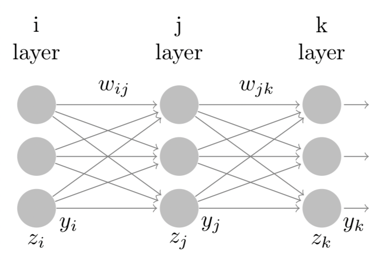
\includegraphics{network}
\end{center}

For convenience, we may consider only one training example and ignore the bias term. Forward propagation of the input $z_i$ is done as follows. Where $g(z)$ is some differentiable function (e.g. the logistic function).

\begin{equation*}
\begin{aligned}
y_i = g(z_i)\\
z_j = \sum_{i}^{}w_{ij}y_i\\
y_j = g(z_j)\\
z_k = \sum_{j}^{}w_{jk}y_j\\
y_k = g(z_k)
\end{aligned}
\end{equation*}

Derive the general expressions for the following partial derivatives of an error function $E$, also sime differentiable function, in the feed-forward neural network depicted. In other words, you should derive these partial derivatives into "computable derivative" (e.g., $\frac{\partial E}{\partial y_k}$ or $\frac{\partial z_k}{\partial w_{jk}}$).
\begin{center}
(a) $\frac{\partial E}{\partial z_k}$
(b) $\frac{\partial E}{\partial z_j}$
(c) $\frac{\partial E}{\partial w_{ij}}$
\end{center}

(a) $\frac{\partial E}{\partial z_k} = \frac{\partial E}{\partial y_k}\frac{\partial y_k}{\partial z_k} = \frac{\partial E}{\partial y_k}g'(z_k)$

(b) $\frac{\partial E}{\partial z_j} = \frac{\partial E}{\partial y_j}\frac{\partial y_j}{\partial z_j} = g'(z_j)\sum_{k}\frac{\partial E}{\partial z_k}\frac{\partial z_k}{\partial y_j} = g'(z_j)\sum_{k}\frac{\partial E}{\partial y_k}g'(z_k)w_{jk}$

(c) $\frac{\partial E}{\partial w_{ij}} = \frac{\partial z_j}{\partial w_{ij}}\frac{\partial E}{\partial z_j} = y_i g'(z_j)\sum_{k}\frac{\partial E}{\partial y_k}g'(z_k)w_{jk}$
\end{document}
